\documentclass[10pt,a4paper]{article}
\usepackage{kotex}
\setmainhangulfont{malgun.ttf}[Path=C:/Windows/Fonts/,BoldFont=malgunbd.ttf]
\setsanshangulfont{malgun.ttf}[Path=C:/Windows/Fonts/,BoldFont=malgunbd.ttf]
\setmonohangulfont{malgun.ttf}[Path=C:/Windows/Fonts/,BoldFont=malgunbd.ttf]
\usepackage[margin=2.2cm]{geometry}
\usepackage{amsmath,amssymb}
\usepackage{booktabs,graphicx,xcolor,enumitem,caption}
\usepackage[hidelinks]{hyperref}
\usepackage{float}
\captionsetup{font=small}
\setlength{\parskip}{3pt}
\newcommand{\pend}[1]{\textcolor{red}{\textbf{[#1]}}}
\newsavebox{\claimsave}
\newenvironment{claimbox}[1]{\begin{lrbox}{\claimsave}\begin{minipage}{0.94\linewidth}\textbf{#1}\par\vspace{2pt}}{\end{minipage}\end{lrbox}\begin{center}\setlength{\fboxsep}{6pt}\fcolorbox{blue!50!black}{blue!4}{\usebox{\claimsave}}\end{center}}

\linespread{1.15}
\renewcommand{\tablename}{표}
\renewcommand{\figurename}{그림}
\title{\textbf{구조를 이해하는 초안 제안:\\HTML의 모양을 이용해 어디서 베낄지 고르기}}
\author{GenerativeUI 프로젝트, KSEF26 --- 연구 주장 노트, 한국어판}
\date{2026-11-07}
\begin{document}
\maketitle

\begin{claimbox}{핵심 주장}
\begin{enumerate}[leftmargin=1.4em,itemsep=2pt]
\item 이미 알려진 기술 두 가지, 즉 비슷한 예시 화면을 주는 것과 그 예시 조각을 초안으로 다시 쓰는 것을 합치면, 작은 모델이 정확도 손실 없이 화면을 약 11배 빨리 만든다. 화면 절반이 보이는 시간은 48.2초에서 3.3초로 줄었다.
\item 남은 낭비는 초안을 \emph{어디서} 베끼느냐에 있다. HTML에는 같은 짧은 조각이 여러 번 나오기 때문에, 기존 방법은 엉뚱한 곳에서 이어 쓰는 일이 잦다.
\item HTML 구조를 따라가는 간단한 규칙은 더 좋은 위치를 골라 모델 호출을 7.9\% 줄인다. 일반적인 개선 방법보다 낫다. 매번 가장 좋은 위치를 고르면 호출이 1.76배 줄어드므로, 위치를 학습으로 고를 여지가 크다.
\item 가장 빠른 예시를 학습으로 고르는 방법과, 같은 화면을 만드는 초안을 받아 주는 방법도 시도했다. 둘 다 효과가 작거나 미리 예측할 수 없었다.
\end{enumerate}
\end{claimbox}

\section{문제}
\emph{생성형 UI}에서는 사용자가 ``회원가입 버튼이 있는 로그인 화면'' 같은 요청을 입력하면 언어 모델이 그 화면의 HTML 코드를 쓴다. HTML은 웹 페이지를 적는 언어이고, CSS는 그중 색과 크기와 위치를 정하는 부분이다. 브라우저가 코드를 그림으로 그리고, 사용자는 그 그림만 본다.

모델은 코드를 작은 조각 하나씩 쓴다. 이 조각을 \emph{토큰}이라고 하며 대략 짧은 단어나 글자 몇 개에 해당한다. 토큰 하나마다 모델을 한 번 돌려야 한다. 그래서
\begin{equation}
\text{기다리는 시간} \;\approx\; \text{모델 호출 횟수} \times \text{호출 한 번의 시간}.
\end{equation}
말로 풀면, 사용자를 덜 기다리게 하려면 모델 호출 횟수를 줄여야 한다. 보통 생성은 토큰 하나에 호출 한 번이므로, 토큰 1000개짜리 화면은 1000번 호출해야 한다.

모델은 Google이 공개한 언어 모델 묶음인 Gemma~4를 썼다. 결과 대부분은 가장 작은 모델인 E2B로 얻었고, 이하 작은 모델이라고 부른다. 아무 도움 없이 쓰면 화면 하나에 약 1분이 걸린다.

\section*{1부. 확인한 것}

\section{시스템 성과: 정확도는 그대로, 약 11배 빠르게}
이미 알려진 두 가지 방법이 대부분의 일을 한다.
\begin{itemize}[itemsep=1pt]
\item \textbf{예시 주기.} 정답과 비슷한 기존 화면 세 개를 요청에 함께 넣는다. 그러면 모델이 많이 베끼고 코드도 짧게 쓴다.
\item \textbf{예시를 초안으로 다시 쓰기.} 한 번에 토큰 하나를 쓰는 대신, 예시에서 다음 토큰 여러 개를 \emph{초안}으로 가져와 모델이 한 번의 호출로 초안 전체를 확인하게 한다. 여러 토큰을 확인하는 비용은 하나를 쓰는 비용과 비슷하다. 모델은 자기 생각과 맞는 앞부분만 받아들이므로 출력은 바뀌지 않는다.
\end{itemize}
초안으로 얻는 속도 향상은 대략 다음과 같다.
\begin{equation}
\text{몇 배 빨라지나} \;\approx\; \text{모델이 호출 한 번에 받아들이는 평균 토큰 수}.
\end{equation}
말로 풀면, 호출 한 번에 토큰 1개 대신 5개를 받아들이면 생성이 약 5배 빨라진다.

\begin{table}[H]\centering\small
\caption{작은 모델, 시험 화면 10개의 중앙값. ``몇 배 빨라졌나''는 첫 줄과 비교한 값이다. 출처: \texttt{runs/poc/E2B\_Ctable.md}, \texttt{runs/poc/E2B\_perc.md}.}\label{tab:main}
\begin{tabular}{lrrrcc}
\toprule
방법 & 화면 전체 & 화면 절반이 보일 때 & 몇 배 빨라졌나 & 체크리스트 & 요소 일치도\\
\midrule
예시 없음, 보통 생성 & 59.4초 & 48.2초 & 1.0 & 87\% & 48\%\\
단어로 찾은 예시, 보통 생성 & 27.1초 & 20.3초 & 2.2 & 100\% & 50\%\\
단어로 찾은 예시, 초안 재사용 & 6.6초 & 4.5초 & 9.0 & 100\% & 50\%\\
구조로 찾은 예시, 초안 재사용 & 5.3초 & 3.3초 & \textbf{11.2} & 100\% & 51\%\\
\bottomrule
\end{tabular}
\end{table}

\emph{체크리스트}는 주 정확도 점수다. 요청에는 ``Cancel 버튼'' 같은 요소가 두세 개 들어 있고, 만든 화면에 그 요소가 하나하나 있는지 확인한다. \emph{요소 일치도}는 만든 화면과 정답 화면의 요소를 비교한다. 두 점수 모두 같거나 올랐다. 이 결과는 기존 기술을 조합한 것이며, 우리의 새 기여가 아니라 출발점이라는 점을 분명히 한다.

\section{구조로 찾은 예시는 속도는 같고 요구사항을 더 많이 채운다}
보통의 검색은 요청과 단어가 맞는 예시를 찾는다. 우리는 요청을 읽고 정답 화면의 \emph{구조}를 예측하는 간단한 모델을 학습했다. 예를 들면 ``위쪽 제목 막대, 가운데 목록, 아래쪽 버튼 두 개'' 같은 예측이다. 그리고 구조가 가장 비슷한 기존 화면을 골랐다.
\begin{itemize}[itemsep=1pt]
\item 초안 재사용을 쓰는 50개 화면에서, 구조로 찾은 예시는 체크리스트를 94.8\%에서 98.2\%로 올렸다. 향상은 3.3\%포인트이고 95\% 신뢰구간이 0.2에서 7.2\%포인트이므로 운이라고 보기 어렵다. 시간은 5.6초 대 5.7초로 같았다.
\item 반대 결과도 있다. 모델 없이 첫 예시를 그대로 답으로 복사하면, 개발용 화면 100개에서 구조 검색 쪽 체크리스트가 8.3\%포인트 \emph{낮았다}. 구조 예시는 복사기가 아니라 모델에게 도움이 된다.
\end{itemize}

\section{코드 겹침이 큰 예시는 오히려 느리고, 가장 빠른 예시는 미리 맞히기 어렵다}
정답과 코드가 가장 많이 겹치는 예시가 가장 빠를 것이라고 예상했다. 결과는 반대였다. 겹침이 가장 큰 예시를 고르면 화면당 1.40초 느려졌고, 95\% 신뢰구간은 0.41초에서 2.42초였다. 그런 예시는 대체로 더 길다.

다음으로 요청 50개마다 예시를 여섯 가지로 바꿔 모두 시간을 쟀다.
\begin{itemize}[itemsep=1pt]
\item 어떤 예시를 주느냐가 크게 중요하다. 단어 검색 1위 예시는 평균 9.33초, 여섯 개 중 가장 빠른 예시는 4.73초로 37\% 짧았다.
\item 이 차이의 4분의 3은 모델이 쓴 답의 길이에서, 4분의 1은 초안을 얼마나 받아들였는지에서 나온다.
\item 그러나 생성 전에 알 수 있는 어떤 특징도 시간을 잘 예측하지 못했다. 모든 특징의 상관계수가 0.13 이하였다. 상관계수는 두 값이 함께 움직이는 정도를 $-1$에서 $1$ 사이 숫자로 나타낸 것이다.
\item 학습한 선택 모델은 격차의 13\%만 메웠고, 이 향상도 통계적으로 뚜렷하지 않았다.
\end{itemize}
그래서 빠른 예시를 학습으로 고르는 것은 핵심 기여로 삼지 않는다.

\section{효과가 작았던 두 가지 시도}
\paragraph{같은 화면을 만드는 초안 받아 주기.} 서로 다른 코드가 같은 화면을 그릴 수 있다. 예를 들어 \texttt{<p>Hello</p>}와 \texttt{<p>Hello}는 똑같이 보인다. 그래서 코드가 달라도 같은 화면을 만드는 초안이면 받아 주는 방법을 시도했다. 하지만 거절된 초안 중 실제로 같은 화면을 만드는 것은 6\%에서 18\%뿐이어서 이 방법의 여지는 작다.

\paragraph{스타일 코드 순서 바꾸기.} 모델은 보통 스타일 코드를 맨 앞에 몰아 쓰기 때문에 화면이 오래 비어 있다. 각 스타일 규칙을 그것이 처음 쓰이는 부분 바로 앞으로 옮겨도 최종 화면은 똑같다. 보통 생성에서는 효과가 있었다. 화면 절반이 전체 시간의 81\%가 아니라 67\% 지점에서 보였다. 초안 재사용과 함께 쓰면 효과가 없었다. 화면 절반이 3.5초가 아니라 4.0초에 보였다.

\section*{2부. 새로 제안하는 방향: 구조를 이해하는 초안 위치 선택}

\section{문제: HTML은 같은 조각을 반복한다}
초안을 만들 때 기존 방법은 모델이 방금 쓴 몇 토큰을 보고, 예시에서 같은 토큰을 찾아, 그 뒤를 베낀다. 그런데 HTML에서는 \texttt{"><div class="} 같은 짧은 조각이 한 예시 안에도 여러 번 나온다. 그래서 기존 방법은 엉뚱한 곳으로 건너뛰어 잘못된 위치에서 이어 쓰는 일이 잦고, 모델은 그 초안을 거절한다.

이 선택을 식으로 쓰면 다음과 같다.
\begin{equation}
\text{가장 좋은 위치} \;=\; \text{예시 안에서, 이어 쓰면 모델이 가장 많은 토큰을 받아들일 위치}.
\end{equation}
말로 풀면, 예시 안에서 베끼기 시작할 수 있는 모든 위치 중 가장 길게 받아들여질 초안을 주는 곳을 고르고 싶다. 기존 방법은 그저 가장 최근에 글자가 맞은 곳을 고른다.

\section{근거}
이미 얻은 출력을 다시 재생하면서, 위치를 고르는 방법마다 모델 호출이 몇 번 필요한지 셌다. 이것은 이상적인 보통 생성을 기준으로 받아들여지는 토큰을 센 분석이며, 실제 시간을 잰 것은 아니다.
\begin{enumerate}[itemsep=1pt]
\item \textbf{재생은 정확하다.} 기존 방법에 대해, 실제 기록의 모델 호출 횟수를 화면 10개 중 10개에서 똑같이 재현했다.
\item \textbf{위치 선택은 큰 지렛대다.} 매번 가장 좋은 위치를 고르면 모델 호출이 1.76배 줄어든다. 기존 방법이 거의 받아들이지 못한 단계의 46\%는, 예시 안의 다른 위치였다면 2토큰 이상 받아들였을 것이다.
\item \textbf{HTML 구조가 일반적인 개선보다 낫다.} 지금 HTML 구조의 어디에 있는지도 확인하는 규칙이 있다. 예를 들면 ``방금 요소 하나를 닫았으니 예시에서 다음 요소를 이어 쓴다''는 식이다. 이 규칙은 호출을 7.9\% 줄이고, 95\% 신뢰구간은 6.4\%에서 9.5\%다. 더 긴 글자열로 맞추는 방법은 4.0\%, 여러 후보의 다수결은 0.7\%만 줄인다. 요청마다 가장 좋은 일반 방법과 비교해도, 구조 규칙은 화면당 4.4번에서 8.9번의 호출을 95\% 신뢰도로 아낀다. 늘어난 수용 토큰의 약 60\%는 한 요소가 끝나고 다음 요소가 시작되는 지점에서 나왔다.
\item \textbf{학습할 여지가 남아 있다.} 규칙을 쓴 뒤에도 가장 좋은 위치까지의 격차 중 81\%에서 85\%가 남는다.
\end{enumerate}

\begin{figure}[H]\centering
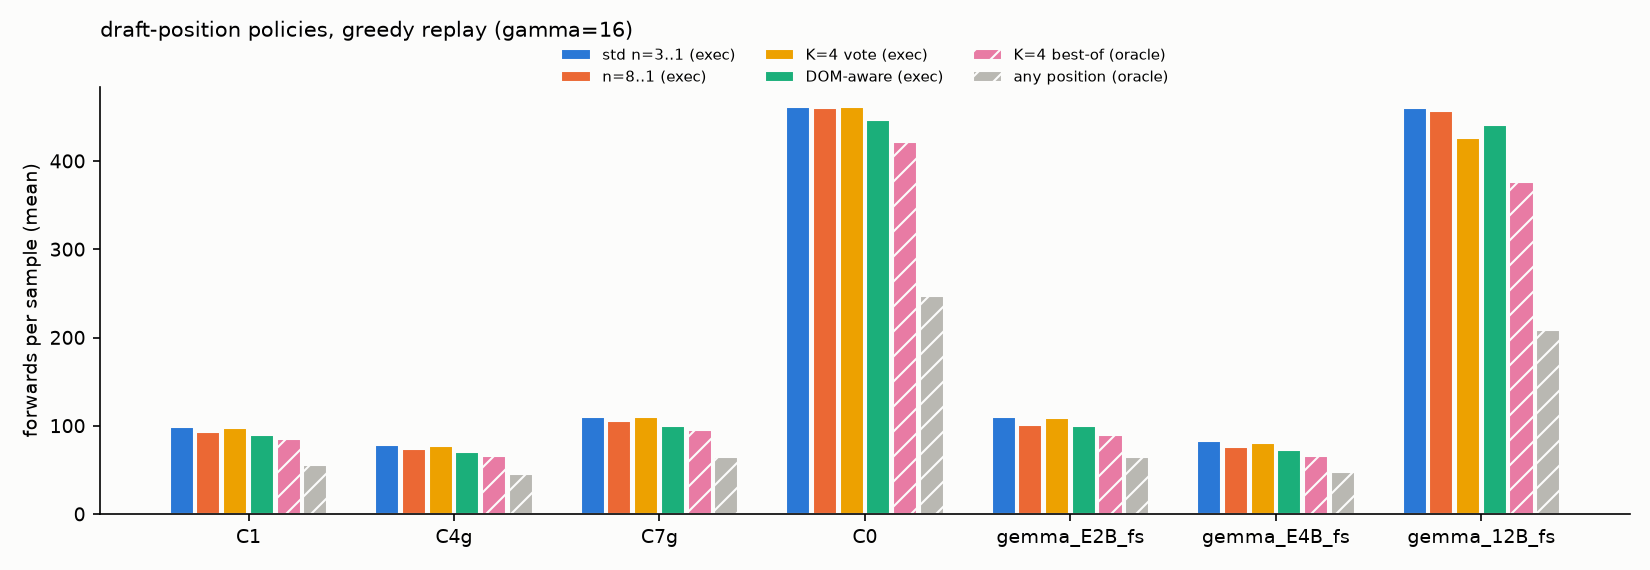
\includegraphics[width=\linewidth]{../runs/study/figures/draft_sim.png}
\caption{위치를 고르는 방법별 화면당 모델 호출 횟수. 낮을수록 좋다. 각 묶음에서 파란색은 기존 방법, 초록색은 구조 규칙, 회색은 가장 좋은 위치를 매번 고른 경우다. 왼쪽 네 묶음은 예시를 달리한 작은 모델이고, 오른쪽 세 묶음은 Gemma~4의 작은, 중간, 큰 모델이다.}\label{fig:sim}
\end{figure}

\section{제안하는 기여}
\begin{enumerate}[itemsep=1pt]
\item \textbf{문제 정의.} HTML의 반복 구조 때문에 글자 맞추기로 만든 초안이 잘못된 위치에서 시작하는 일이 잦고, 남은 낭비의 대부분이 여기에 있음을 보인다.
\item \textbf{학습.} 지금의 HTML 구조 상태와 모델의 내부 상태를 보고 ``이 위치에서 몇 토큰이 받아들여질지''를 예측하는 위치 선택 모델을 만든다.
\item \textbf{사용.} 모델은 지금처럼 모든 초안을 그대로 확인하므로 출력은 바뀌지 않는다. 바뀌는 것은 초안을 고르는 방법뿐이다.
\end{enumerate}

\paragraph{다음 단계.} 위치 선택 모델을 개선한다. 그 위치가 직전 초안을 이어 가는지 알려 주고, 개수를 맞히는 대신 위치의 순위를 매기도록 학습시키고, 실제 실행 데이터로 학습시킨다. 그래픽 카드에서 실제 시간을 잰다. 큰 모델에서 효과가 사라진 원인을 확인한다.

\section{시험 방법}
시험 세트는 Screen2Words로 만들었다. Screen2Words는 실제 안드로이드 앱 화면 약 22{,}000개와 화면마다 사람이 쓴 설명 다섯 개를 모은 공개 자료다. 문항 하나는 요청 하나와 정답 화면의 HTML이다. 요청에는 목적과 핵심 요소 두세 개가 들어가지만 개수나 긴 원문은 없어서, 정답이 될 수 있는 화면이 여럿이다. 정답 화면은 체크리스트를 100\% 통과하고, 고정된 틀은 8\%, 가장 비슷한 기존 화면을 베끼면 37\%를 통과한다. 시험용 화면 500개, 개발용 화면 100개, 예시용 화면 14{,}522개를 쓰며, 세 묶음 사이에 같은 앱은 없다.

\section{한계}
\begin{itemize}[itemsep=1pt]
\item 속도는 화면 10개에서 50개로 쟀다. 화면 10개에서는 체크리스트가 거의 늘 100\%라서 방법을 잘 구분하지 못한다.
\item 초안 재사용은 출력을 바꾸지 않아야 하지만, 4비트와 16비트 계산의 반올림 때문에 10개 중 7개가 보통 생성과 조금 달랐다. 또 모델을 공식 형식과 비슷한 4비트 형식으로 돌렸다.
\item 구조 규칙은 작은 모델과 주 실험의 중간 수준 요청에서만 뚜렷하게 나았다. 자세한 요청과 큰 모델에서는 우위가 통계적으로 뚜렷하지 않았다.
\item 처음 학습한 위치 선택 모델은 아직 간단한 규칙보다 못하다. 호출 감소가 6.6\%로, 규칙의 7.9\%보다 작다.
\item 위치 선택 결과는 재생으로 센 모델 호출 횟수이며, 실제 시간은 아직 재지 않았다.
\end{itemize}

\end{document}
